\documentclass[12pt,a4paper,oneside,titlepage,draft]{extreport}

% Ничего местами не менять! Всё, что находится после знака процента, на печать не влияет.

\usepackage{hyperref}
\usepackage{xcolor}

\definecolor{linkcolor}{HTML}{000000}
\definecolor{urlcolor}{HTML}{000000}
\hypersetup{pdfstartview=FitH,linkcolor=linkcolor,urlcolor=urlcolor,colorlinks=true}

\usepackage[cm-default]{fontspec}
\usepackage{xunicode}
\usepackage{xltxtra}

\usepackage{polyglossia}
\setdefaultlanguage{russian}
%\setotherlanguage{english}

\setmainfont{XITS}
%\setsansfont{PT Sans}
%\setmonofont{PT Mono}

\usepackage{graphicx}
\usepackage[left=3.00cm, right=3.00cm, top=2.00cm, bottom=2.00cm]{geometry}

\parindent=1.25cm
\usepackage{setspace}
\setstretch{1.5}
%\sloppy

\usepackage{gensymb}

% «  »

\begin{document}
	
	\begin{titlepage}
		\begin{center}
		
			{Министерство культуры Российской Федерации}		
		
			{ФГБОУ ВО «Санкт-Петербургская государственная консерватория
			им.~Н.~А.~Римского-Корсакова»}
		
			{Кафедра \emph{<оркестровых струнных инструментов?>} \marginpar{{\Large \textbf{?}}}}
	
	%		{\hfill\hrulefill\hrulefill\hfill}
	
		\vfill
		\vfill
		\vfill
				\begin{Large}
				{\textbf{Горячев Сергей \emph{<Отчество>} \marginpar{{\Large \textbf{?}}}}}
				\end{Large}
								

				%{{\small \textit{(исправленный от \today)}}}	

		\vfill
		
				{\large {\textbf{Виолончельные миниатюры в творчестве русских композиторов XIX века и их значение в педагогической практике}}}
				
		\vfill
		
				\normalsize
		
				{Выпускная квалификационная работа\\
по направлению подготовки (специальности)\\
код специальности –-- «Наименование специальности»\\
специализация (профиль) --– «наименование специализации (профиля)» \marginpar{{\Large \textbf{?}}}}
    		\vfill		
		\vfill		
		\vfill
		\vfill
		\end{center}
		\begin{flushright}
			Руководитель --- \\
			ученая степень и ученое звание \\
			\textbf{Фамилия И.О.} \marginpar{{\Large \textbf{?}}} \\
%		
%		\medskip 			
%		
%			\emph{Проверил:}\\
%			д. т. н., профессор\\
%			Нырцов М. В.
		\end{flushright}
	\vfill
	\vfill
		\begin{center}
			{Санкт-Петербург \\ 2018}
		\end{center}		
	\end{titlepage}
	
	\tableofcontents
	
	\chapter*{Введение}
		\addcontentsline{toc}{chapter}{Введение}
	
	\begin{enumerate}
	\item Обоснование выбора темы
	\item Актуальность данной темы
	\item Формулировка изучаемой проблемы
	\item Определение объекта и предмета исследования
	\item Постановка целей и задач исследования
	\item Краткая характеристика используемой литературы
	\end{enumerate}	
	
		
	
	\chapter*{Основная часть}
		\addcontentsline{toc}{chapter}{Основная часть}
		
		Осветить тему и вопросы, заданные во введении.
		
		20–25 страниц во всём документе, включая титульный лист, содержание и список литературы, кроме приложения)

	\section*{Глава 1. Виолончельное искусство в России I половины XIX века}
		\addcontentsline{toc}{section}{Глава 1. Виолончельное искусство в России I половины XIX века}
		
		Переломным моментом в истории развития русской музыки вообще являются шестидесятые годы XIX века, когда вскоре после отмены крепостного права и проведения ряда либеральных реформ Русским музыкальным обществом были открыты Санкт-Петербургская (а позднее и Московская) консерватории, появилось множество талантливых выходцев из разночинных кругов, создавались творческие коллективы наподобие «Могучей кучки». %\cite{ginzburg:2}. 		
		Именно тогда виолончельное искусство в нашей стране достигло наивысшего расцвета, представив миру таких замечательных музыкантов, как К.~Ю.~Давыдов, А.~В.~Вержбилович, А.~А.~Брандуков и других. 
		
		До этого времени развитие шло в основном через разного рода крепостные оркестры (которых к началу века насчитывалось несколько сотен), влияние иностранной музыки и приезжих музыкантов, любителей и воспитанников театральных школ:
		
		\begin{quotation}
		\textit{К этому времени, то есть к 60-м годам, почва для 
создания в России национальной виолончельной школы как
единого направления была вполне подготовлена; достаточно
вспомнить достижения талантливых русских виолончелистов
конца XVIII и первой половины XIX столетий — выходцев из
крепостной или разночинной среды — Хорошевского, 
Волкова, Татаринова, Сухова, Мешкова, Терентьева, Агапьева,
Лобкова, Подобедова, а также представителей 
любительских кругов — Матвея Вельгорского и Николая Голицына.} %\citep{ginzburg:3}
		\end{quotation}
		
		Исполнительское искусство первой 
четверти века еще продолжает идти по пути накопления творческого опыта, освоения жанров и форм музыкальной практики, вызревания национальных особенностей исполнительской школы.				
		К середине XIX века формируются основные особенности, традиции русского смычкового искусства, направленные на наиболее полное выражение музыкальной мысли, уход от излишней виртуозности, стремление к использованию её в 
качестве средства выразительности, служащего художественной
правдивости и убедительности трактовки исполняемых 
произведений.
		
		В конце XVIII --- начале XIX века одним из лучших считался оркестр крепостного театра графа Н. П. Шереметева (учившегося игре на виолончели у Ивара), в репертуар которого входили симфонии Моцарта, Гайдна, множество опер того времени. В этом оркестре можно упомянуть вольнонаёмного немецкого виолончелиста \emph{Иоганна Фациуса}, крепостных \emph{К. Четверикова, Н. Чухнова,} учителем которых был Фациус, и \emph{Д. Стрехвалова.}
		
Находясь в Москве на службе, Фациус не прекращал концертной деятельности в течение порядка 25 лет. Он играл 
преимущественно свои сочинения, среди которых были виолончельные
концерты, сонаты, дуэты, исполнявшиеся также при участии его вышеназванных учеников и самого Шереметева.%\citep{ginzburg:2}

Позднее оркестр был распущен из-за смерти актрисы и певицы театра П. И. Жемчуговой (1768--1803), которой Шереметев дал вольную.

Также с XVIII века большое распространение получили домашние ансамбли --- от случайных дуэтов или других составов
(в том числе и с участием певцов) до хорошо сыгравшихся квартетов, в которых могли участвовать и некоторые иностранные музыканты (например, выступавший при дворе Екатерины II квартет в составе скрипачей Дица и Тевеса, альтиста Штокфиша и виолончелиста Дельфино, игравшего в La Scala). Использованию
виолончели в квартетах или в сольном исполнительстве 
предшествовало её применение в роли баса в различных домашних 
ансамблях.

О профессиональном уровне русского квартетного 
исполнительства того времени свидетельствует присутствие в русских нотных каталогах большого количества камерных произведений Гайдна, Моцарта и Бетховена, а также Боккерини, Пуньяни, Стамица и других композиторов. Практически одновременно 
появляется и целый ряд русских произведений для квартета,
как, например, С. Танеева, И. Воробьева, А. Алябьева, в которых чётко прослеживается использование интонаций
русской народной песни, формировавшее особенности исполнительского стиля в 
квартетном и сольно-концертном жанрах.

Также известны квартеты начала XIX века, в состав которых входили 
музыканты-профессионалы, как, например, московский квартет в
составе Кубишты, Шольца, Конюса и Марку, квартет В. А. Всеволожского в Москве. Неоднократно участвовали в русских квартетах первых десятилетий
XIX века виолончелисты \emph{Н. Голицын, М. Вельгорский,} известный немецкий виолончелист \emph{Б. Ромберг}, польский виолончелист \emph{Н. Зигмунтовский}, чешские виолончелисты \emph{Ф. Керцель} (организовавший в Москве первое
исполнение гайдновской оратории «Семь слов Христа» и, вероятно, бывший учредителем 
Московского музыкального училища в 1773 г.), \emph{Я. Мареш, Й. Фиала} и другие.

В Петербурге и Москве в дворянском и купеческом сословиях создавались любительские музыкальные клубы, организовывавшие концерты с участием видных русских и иностранных музыкантов. Здесь ставились оперы, исполнялись произведения наподобие «Stabat mater» Перголези,
кантаты Березовского. В 1778 году в Петербурге был учрежден «Новый 
музыкальный клуб», в концертах которого принимали участие неы
только музыканты-любители, но и Бортнянский, Гесслер и др.
В Москве в конце XVIII века была организована 
«Музыкальная академия», по характеру своей деятельности 
сходная с петербургскими клубами.

К числу выпускников театральных школ и училищ следует отнести московских виолончелистов Куликова, Наврозова, Соколова, петербургского 
виолончелиста П. И. Григорьева, А. Маурера.

Стоит отметить служившего в Московском театре виолончелиста \emph{Ивана Осиповича Лобкова.} Он неоднократно принимал 
участие в концертах своих товарищей, например, в концертах
служившего с ним в театре скрипача Полякова. В одном из
таких концертов (23 марта 1822 г.) Лобков исполнил рондо A-dur Ромберга.
В его репертуар также входили сольные 
вариации, балетные дивертисменты на 
мотивы русских песен и плясок.

Отличным виолончелистом был младший современник Лобкова \emph{Иван Корнилович Подобедов,} происходивший из крепостных.
С 1840 года он состоял действительным членом Петербургского филармонического общества, с 1836 года на протяжении многих лет преподавал в театральном училище. К сожалению, до нашего времени не дошли виолончельные сочинения
Подобедова, однако известны его несколько фортепианных произведений.
		
%%%%%%%%%%%%%%%%%%%%%%%%%


	
	\section*{Глава 2. К. Ю. Давыдов и его ученики}
		\addcontentsline{toc}{section}{Глава 2. К.~Ю.~Давыдов и его ученики}
				
%	\begin{figure}[h]
%	\centering
%	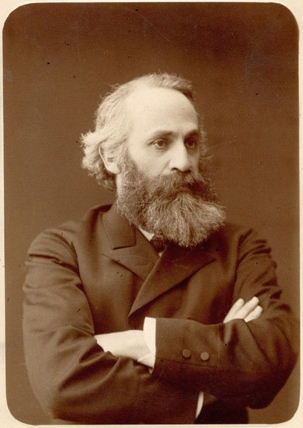
\includegraphics[scale=1]{davydov.png}
%	\caption{f}
%	\end{figure}	

		Одним из самых ярких виолончелистов в истории русской и европейской музыки считается директор Санкт-Петербургской консерватории \emph{Карл Юльевич Давыдов (1838--1889).} Под руководством выдающегося музыканта, солиста оркестра Большого театра Г. Шмита, он сумел добиться блестящих технических результатов уже в раннем возрасте (и в 14 лет дать свой первый публичный концерт в Москве). 
		
		На своём посту директора консерватории, помимо насыщенной концертной, организаторской и композиторской деятельности он очень много времени уделял педагогике:
		
		\begin{quotation}
		\textit{Созданию и развитию отечественной виолончельной 
школы Давыдов посвятил лучшие годы своей жизни. За время
25-летней деятельности в качестве профессора 
Петербургской консерватории Давыдов воспитал значительное число
виолончелистов, работа которых в различных русских 
городах способствовала дальнейшему развитию виолончельного
искусства в стране. Среди его учеников можно назвать
А. Вержбиловича, Д. Бзуля, С. Морозова, А. Воробьева,
Н. Логановского, А. Глена, Ф. Мулерта, А. Кузнецова,
И. Шмидта, Я. Розенталя, П. Федорова, А. Вербова, В. Гу-
тора, Ю. Бологовскую, Н. Потапова и многих других.}
		\end{quotation}
		
		Одним из его важнейших педагогических трудов является так называемая «Школа», сборник небольших этюдов-пьес в сопровождении второй виолончели или фортепиано, каждый из которых посвящён определённой технической задаче.
		
		\begin{quotation}
		«Школа» начинается с описания так называемой 
постановки виолончелиста (ее характеризуют условия, 
обеспечивающие наиболее естественные и свободные движения
играющего) 3, 'правил ведения смычка (а также функций
отдельных частей руки, ведущей смычок) и положения левой
руки на грифе. Затем детально рассматривается первая
позиция; при этом четко дифференцируются широкое и узкое
расположения пальцев на грифе, что является одной из
основных и специфических предпосылок к достижению 
чистой интонации на виолончели. В первом же разделе 
«Школы» описываются элементарные штрихи с использованием
различных частей смычка; вскрываются закономерности
равномерного и неравномерного движения смычка. С целью
1 Эта точка зрения сохранилась и в советской педагогической 
практике. Такие произведения, как виолончельные концерты Ромберга, видный
советский методист Б. А. Струве относил к разделу 
«художественно-педагогической: литературы и подчеркивал их значение в процессе 
обучения молодых музыкантов.
2 Во вторую часть «Школы» должны были войти более сложные 
элементы виолончельной техники (использование верхнего регистра, ставка,
двойные ноты, флажолетная техника, сложные штрихи и т. д.) и более
сложные музыкальные задания. Отсутствие второй части в большой мере
компенсируется в педагогической практике изучением концертов и пьес
Давыдова, которым свойственно единство художественного и 
педагогического значения.
3 Общепринятый в настоящее время и наиболее рациональный способ
игры на виолончели со шпилем был закреплен в виолончельной практике
в значительной мере благодаря Давыдову, на страницах своей «Школы»<
решительно выступившему в пользу его применения (см. Книгу первую
«Истории виолончельного искусства». М.—Л., 1950, стр. 36—37).
100концентрации внимания ученика на данной штриховой
трудности, «неравномерным» штрихам 'предпосылаются 
соответствующие упражнения на открытой струне. 
Значительное внимание в этом разделе уделяется технике переходов
смычка со струны на струну.
Второй раздел «Школы» посвящен первым четырем 
позициям К Здесь (в сущности, впервые в смычковой 
педагогической литературе) излагается методически обоснованная
система смены позиций; система эта сохранила свое значение
и в современной виолончельной практике.
В третьем разделе «Школы» рассматриваются более 
высокие позиции (до седьмой включительно) и приводятся все
двухоктавные (мажорные и минорные) гаммы.
Гаммы имеют два вида аппликатуры — с применением
открытых струн и без них. Гаммы с используемой 
Давыдовым стандартной для всех тональностей аппликатурой без
применения открытых струн2 дают незаменимый материал
для тренировки в смене позиций, в чередовании узкого и 
широкого расположения 'пальцев; они способствуют выработке
чистой интонации и ровности звучания.
Основным достоинством «Школы», способствующим ее
широкому применению в советской педагогической практике,
является характерное для Давыдова-педагога прогрессивное
стремление к единству художественного и 
технического развития учащегося. Стремление это
ярко сказывается в подборе нотного материала к «Школе»,
который, в основном, состоит из небольших этюдов-пьес, 
соответствующих определенным техническим заданиям и в то
же время обладающих несомненными художественными 
достоинствами. Эти этюды-пьесы (Давыдов называет их 
примерами) написаны с сопровождением второй виолончели или
фортепиано3, что -повышает их музыкальную ценность и
содействует приобретению навыков игры в ансамбле. Таким
образом, развитие технических навыков идет одновременно
и в связи с. развитием музыкальности учащегося, его мело-
1 Понимая позиции» как условное разделение грифа, Давыдов связал это разделение е ладовым чувством играющего: его классификация
позиций строится по ступеням мажорной диатонической гаммы от данной
открытой струны.
2 Пятнадцать звуков двухоктавной гаммы разбиваются Давыдовым
на пять групп по три звука; каждая из этих групп укладывается в одну
лозшшю. Таким образом, мажорная гамма в восходящем движении 
играется следующими пальцами: 1—2 4, 1—2 4, 1 2 4, 1 2 4, 1 3 4. 
Минорная—в восходящем движении: 1, 3 4. 1—2 4, 1 2 4, 1—2 4, 1 3 4, а в
нисходящем: 4, 2—1, 4, 2—'1, 4 2—1, 4 3 1, 4 3 1 (черточка означает
пелотоппое растяжение между 1 и 2 пальцами).
3 Как *;Виолончельные этюды для начинающих» они были переизданы
советским издательством в редакции С. Л. Гинзбурга (Л., 1935).
101дического и гармонического слуха, чувства ритма, чувства
ансамбля и т. д.
Все это способствует сохранению значения «Школы»
Давыдова и в современной педагогической практике.
Методические взгляды Давыдова в значительной степени
могут быть восстановлены также на основе изучения 
аппликатурных, штриховых и динамических обозначений в его
виолончельных концертах и пьесах, в принадлежащих ему
виолончельных переложениях, а также в его редакциях
виолончельных партии концерта Шумана \ первой части IX
концерта Ромберга2, Тарантеллы из концерта Линднера3,
квартетов Бетховена и Шумана4.
		\end{quotation}
		
		\subsection*{Пьесы-посвящения.}
		
		Какая
Пьеса кому посвящена
Про технические сложности
		
		Свой предсмертный цикл из четырёх виолончельных пьес «Силуэты» в сопровождении фортепиано (ор.41, 1887 г.) Давыдов посвятил четырём виолончелистам: участнику квартета Иоахима --– Роберту Гаусману («Утром») и трём своим ученикам --– Александру Вержбиловичу  («Вальс»), Александру Кузнецову  («Ноктюрн»)  и Альфреду Глену  («У озера Лугано»).
		
	
	\section*{Глава 3. Место виолончели в оркестровой и ансамблевой музыки того времени}
		\addcontentsline{toc}{section}{Глава 3. Место виолончели в оркестровой и ансамблевой музыке того времени}
		
		\subsection*{Симфонический оркестр, ансамбли}
		
		\begin{quotation}
		В XVIII веке виолончель получила распространение в 
России не только как оркестровый и ансамблевый, но и как 
сольный инструмент2. Выразительные особенности этого 
инструмента (его задушевная певучесть, близость к тембру 
человеческого голоса), так же как и его технические возможности,
постепенно получают все более широкое признание и 
применение з русской музыкальной практике. Сольное использование
виолончели подготавливалось уже в раннем оперном, 
симфоническом и камерном творчестве русских композиторов.
		\end{quotation}

		Однако одну из решающих ролей в развитии виолончельной музыки, её восприятии слушателем сыграло именно использование инструмента в оркестрах, струнных трио, квартетах и ансамблях
		
		\subsection*{Фактура, технические и выразительные приёмы}
		

	\section*{Глава 4. Основные произведения <дискография>}
		\addcontentsline{toc}{section}{Глава 4. Основные произведения <дискография>}
		
		\begin{enumerate}
\item Рахманинов. 2 пьесы 1892г ,ор 2 1)прелюдия , 2) Восточный танец 
\item Аренский. ор 56 ,12 Восточная мелодия 
\item А.Рубинштейн. 3 пьесы 1954г ор 11/3 
\item Чайковский. Andante cantabile TH 63 ,1871 (1888), Pezzo capriccioso 1887 
\item Римский-Корсаков. Серенада ор 37 
\item Глазунов. 2 пьесы ор20 1) мелодия , 2 )Испанская серенада ,Песнь менестреля ор 71 ,Элегия ор17 
\item Ц.Кюи. 2 пьесы 1886г 1) Scherzando 2) Cantabile , Баркарола ор 81 
\item Давыдов. 3 характерные пьесы 1) одиночество ,2) Юмореска 3) Тарантелла .4 пьсы вечернее размышление 1)Воскресное утро 2) У фонтана 3)У колыбели 4 )Сумерки . Силуэты 4 пьесы ,1)утром 2) Вальс 3)Ноктюрн 4)У озера Лугано 
Воспоминание об Ораниенбауме 1)прощание 2) баркарола 
Баллада для виолончели , Романс
\end{enumerate}

	\section*{Глава 5. Педагогическая ценность}
		\addcontentsline{toc}{section}{Глава 5. Педагогическая ценность}
		
		
	
	\chapter*{Заключение}
		\addcontentsline{toc}{chapter}{Заключение}

	\begin{enumerate}
	\item Выводы
	\item Итоги обсуждения поставленной проблемы
	\item Сформулированные результаты исследования
	\end{enumerate}
	
	%\appendix
	
	\addcontentsline{toc}{chapter}{Литература}	
	\bibliographystyle{ugost2008ns}
	\bibliography{biblio}
	
	
	
\end{document}
